
%%%%%%%%%%%%%%%%%%%%%%% file typeinst.tex %%%%%%%%%%%%%%%%%%%%%%%%%
%
% This is the LaTeX source for the instructions to authors using
% the LaTeX document class 'llncs.cls' for contributions to
% the Lecture Notes in Computer Sciences series.
% http://www.springer.com/lncs       Springer Heidelberg 2006/05/04
%
% It may be used as a template for your own input - copy it
% to a new file with a new name and use it as the basis
% for your article.
%
% NB: the document class 'llncs' has its own and detailed documentation, see
% ftp://ftp.springer.de/data/pubftp/pub/tex/latex/llncs/latex2e/llncsdoc.pdf
%
%%%%%%%%%%%%%%%%%%%%%%%%%%%%%%%%%%%%%%%%%%%%%%%%%%%%%%%%%%%%%%%%%%%


\documentclass[runningheads,a4paper]{llncs}


\usepackage{amssymb}
\usepackage{caption}
\usepackage{subcaption}
\captionsetup{compatibility=false}
\usepackage{algorithm}
\usepackage{algorithmic}
\usepackage{array}
\setcounter{tocdepth}{3}
\usepackage{graphicx}
\usepackage[margin=2.5cm]{geometry}

\usepackage{url}
\newcommand{\keywords}[1]{\par\addvspace\baselineskip
\noindent\keywordname\enspace\ignorespaces#1}

\begin{document}

\mainmatter  % start of an individual contribution

% first the title is needed
\title{Optimistic Concurrency Control in a Distributed NameNode Architecture for Hadoop Distributed File System}

% a short form should be given in case it is too long for the running head
\titlerunning{Optimistic Concurrency Control in a Distributed NameNode Architecture for Hadoop Distributed File System}

% the name(s) of the author(s) follow(s) next
%
% NB: Chinese authors should write their first names(s) in front of
% their surnames. This ensures that the names appear correctly in
% the running heads and the author index.
%
%
\author{Qi Qi}
\authorrunning{Optimistic Concurrency Control in a Distributed NameNode Architecture for Hadoop Distributed File System}
% (feature abused for this document to repeat the title also on left hand pages)
\institute{Instituto Superior Técnico - IST (Portugal) \\ Royal Institute of Technology - KTH (Sweden)}
% the affiliations are given next; don't give your e-mail address
% unless you accept that it will be published

%
% NB: a more complex sample for affiliations and the mapping to the
% corresponding authors can be found in the file "llncs.dem"
% (search for the string "\mainmatter" where a contribution starts).
% "llncs.dem" accompanies the document class "llncs.cls".
%

\toctitle{Reliable and Locality-driven scheduling in Hadoop}
\tocauthor{Qi Qi}
\maketitle


\begin{abstract}
The \textit{Hadoop Distributed File System} (HDFS) is the storage layer for Apache Hadoop ecosystem, persisting large data sets across multiple machines. However, the overall storage capacity is limited since the metadata is stored in-memory on a single server, called the \textit{NameNode}. The heap size of the NameNode restricts the number of data files and addressable blocks persisted in the file system.

The \textit{Hadoop Open Platform-as-a-service} (Hop) is an open platform-as-a-Service (PaaS) support of the Hadoop ecosystem on existing cloud platforms including Amazon Web Service and OpenStack. The storage layer of Hop, called the Hop-HDFS, is a highly available implementation of HDFS, based on storing the metadata in a distributed, in-memory, replicated database, called the \textit{MySQL Cluster}. It aims to overcome the NameNode's limitation while maintaining the strong consistency semantics of HDFS so that applications written for HDFS can run on Hop-HDFS without modifications.

Precedent thesis works have contributed for a transaction model for Hop-HDFS. From system-level coarse grained locking to row-level fine grained locking, the strong consistency semantics have been ensured in Hop-HDFS, but the overall performance is restricted compared to the original HDFS.

In this thesis, we first analyze the limitation in HDFS NameNode implementation and provide an overview of Hop-HDFS illustrating how we overcome those problems. Then we give a systematic assessment on precedent works for Hop-HDFS comparing to HDFS, and also analyze the restriction when using pessimistic locking mechanisms to ensure the strong consistency semantics. Finally, based on the investigation of current shortcomings, we provide a solution for Hop-HDFS based on optimistic concurrency control with snapshot isolation on semantic related group to improve the operation throughput while maintaining the strong consistency semantics in HDFS. The evaluation shows the significant improvement of this new model. The correctness of our implementation has been validated by 300+ Apache HDFS unit tests passing.
\keywords{HDFS, MySQL Cluster, Concurrency Control, Snapshot Isolation, Throughput}
\end{abstract}

\section{Introduction}
The \textit{Hadoop Distributed File System} (HDFS) is the storage layer for Apache Hadoop, which enables petabytes of data to be persisted on clusters of commodity hardware at relatively low cost~\cite{borthakur2008hdfs}. Inspired by the \textit{Google File System} (GFS)~\cite{ghemawat2003google}, the namespace, \textit{metadata}, is decoupled from data and stored in-memory on a single server, called the \textit{NameNode}. The file datasets are stored as sequences of blocks and replicated across potentially thousands of machines for fault tolerance.

Built upon the single namespace server (\textit{the NameNode}) architecture, one well-known shortcoming of HDFS is the limitation to growth~\cite{shvachko2010hdfs}. Since the metadata is kept in-memory for fast operation in NameNode, the number of file objects in the filesystem is limited by the amount of memory of a single machine.

The \textit{Hadoop Open Platform-as-a-service} (Hop) is an open platform-as-a-Service (PaaS) support of the Hadoop ecosystem on existing cloud platforms including Amazon Web Service and OpenStack. The storage layer of Hop, called the Hop-HDFS, is a highly available implementation of HDFS, based on storing the metadata in a distributed, in-memory, replicated database, called the \textit{MySQL Cluster}. It aims to overcome the NameNode's limitation while maintaining the strong consistency semantics of HDFS so that applications written for HDFS can run on Hop-HDFS without modifications.

However, in HDFS, the correctness and consistency of the namespace is ensured by atomic metadata mutation~\cite{shvachko2010hadoop}. In order to maintain the same level of strong consistency semantics, system-level coarse grained locking and row-level fine grained locking are adopted in precedent projects of Hop-HDFS, but the overall performance is heavily restricted compared to the original HDFS. Therefore, investigation for better concurrency control methods to improve the performance of Hop-HDFS is the main motivation of this thesis.

\subsection*{Contribution}
In this thesis, we contribute to the following three ways: First, we discuss the architectures of related distributed file systems, including Google File System, HDFS and Hop-HDFS. With focus on their namespace concurrency control schemes, we analyzes the limitation of HDFS's NameNode implementation. Second, we provide an overview of Hop-HDFS illustrating how it overcomes limitations in HDFS. With a systematic performance assessment between Hop-HDFS and HDFS, we discuss the current shortcomings in Hop-HDFS, which motivates this thesis for a better concurrency control scheme. Third, we provide a solution for Hop-HDFS based on optimistic concurrency control with snapshot isolation on semantic related group to improve the operation throughput while maintaining the strong consistency semantics in HDFS. As a proof of concept, the evaluation shows the significant improvement of this new model. The correctness of our implementation has been validated by 300+ Apache HDFS unit tests passing.

\section{Background and Related Work}
\subsection{The Hadoop Distributed File System}
The \textit{Hadoop Distributed File System} (HDFS) is inspired by the Google File System. Initially, HDFS is built for Hadoop Map-Reduce computational framework. With the development of Hadoop ecosystem including HBase, Pig, Mahout, Spark, etc, HDFS becomes the storage layer for all these big data applications. While enabling petabytes of data to be persisted on clusters of commodity hardware at relatively low cost, HDFS aims to stream these large data sets at high bandwidth to user applications. Therefore, like GFS, HDFS is optimized for delivering a high throughput of data at the expense of latency~\cite{white2012hadoop}.

Similar to GFS, HDFS stores metadata and file data separately. The architecture of a HDFS cluster consists of a single \textit{NameNode}, multiple \textit{DataNodes}, and is accessed by multiple \textit{clients}. Files in HDFS are split into smaller blocks stored in \textit{DataNodes}. For fault tolerance, each block is replicated across multiple \textit{DataNodes}. The \textit{NameNode} is a single dedicated metadata server maintaining the namespace, access control information, and file blocks mappings to DataNodes. The entire namespace is kept in-memory, called the \textit{image}, of the \textit{NameNode}. The persistent record of \textit{image}, called the \textit{checkpoint}, is stored in the local physical file system. The modification of the namespace (\textit{image}), called the \textit{journal}, is also persisted in the local physical file system. Copies of the \textit{checkpoints} and the \textit{journals} can be stored at other servers for durability. Therefore, the \textit{NameNode} restores the namespace by loading the checkpoint and replaying the journal during its restart.

\subsection{Hadoop Open Platform-as-a-service and Hop-HDFS}
The \textit{Hadoop Open Platform-as-a-service} (Hop) is an open platform-as-a-Service (PaaS) support of the Hadoop ecosystem on existing cloud platforms including Amazon Web Service and OpenStack. The goal is to automate the installation of both HDFS and Apache YARN so that unsophisticated users can deploy the stack on the cloud easily by a few clicks from our portal website. 

The storage layer of Hop, called the Hop-HDFS, is a new high available model for HDFS's metadata, aiming to overcome the major limitations of HDFS NameNode architecture: (1) the scalability of the namespace - the memory size restricts the storage capacity in the system; (2) the throughput problem - the throughput of the metadata operations is bounded by the ability of the single machine (NameNode); (3) the failure recovery - it takes a long time for the NameNode to restart since it needs to load the checkpoint and replay the edit logs from the journal into the memory.

The architecture of Hop-HDFS consists of multiple \textit{NameNodes}, multiple \textit{DataNodes}, a \textit{MySQL cluster} and is accessed by multiple \textit{clients} as shown in Figure~\ref{fig:hophdfsar}. The design purpose for Hop-HDFS is to migrate the metadata from NameNode to an external distributed, in-memory, replicated database \textit{MySQL Cluster}. Therefore, the size of the metadata is not limited by a single NameNode's heap size so that the scalability problem can be solved. In Hop-HDFS, we have this \textit{multiple stateless NameNodes} architecture so that multiple-writers and multiple-readers are allowed to operate on the namespace to improve the throughput.

\begin{figure}[h!]
	\centering
	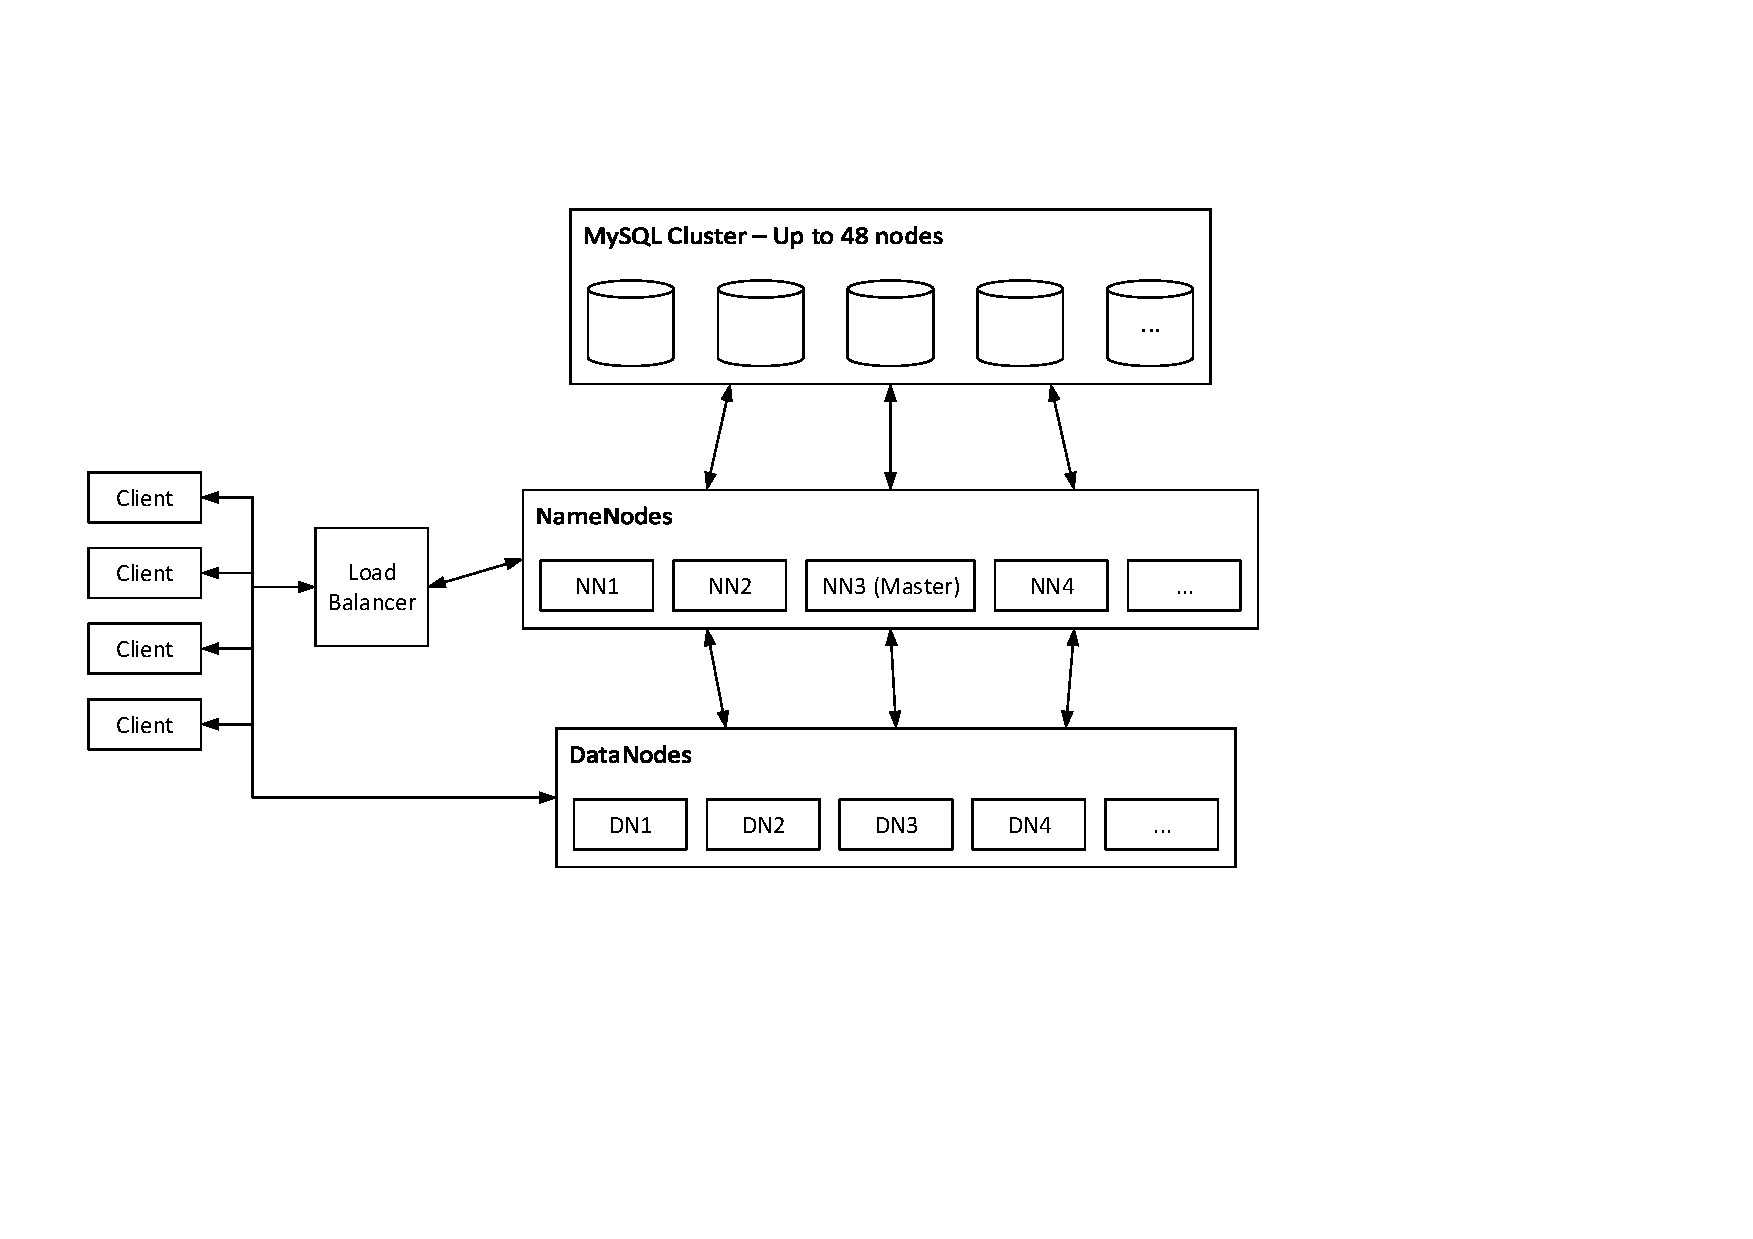
\includegraphics[scale=0.4]{HopHDFSArchitecture.pdf}
	\caption{The Architecture of Hop-HDFS}
	\label{fig:hophdfsar}
\end{figure}

Moreover, the fault tolerance of the metadata is handled by MySQL Cluster, which grantees high availability of 99.999\%. The \textit{checkpoint} and the \textit{journal} for namespace is removed as a result, which reduces the time on writing edit logs as well as restarting new NameNodes on namespace recovery. Note that we have a leader election process in this distributed NameNode architecture. The leader, \textit{master}, will be responsible for tasks like block reporting and statistic functions.

The size of the metadata for a single file object having two blocks (replicated three times by default) is 600 bytes. It requires 60 GB of RAM to store 100 million files in HDFS, 100 million files is also the maximum storage capacity for HDFS in practice. For MySQL Cluster, it supports up to 48 datanodes, which means that it can scale up to 12 TB in size with 256 GB RAM for each node in size. But conservatively, we assume that MySQL Cluster can support up to 3.072 TB for metadata with a data replication of 2, which means that Hop-HDFS can store up to 4.1 billion files. A factor of 40 times increase over Shvachko's estimate~\cite{shvachko2010hdfs} for HDFS from 2010.

\subsection{Fault tolerance in Hadoop}
\subsubsection{Detection of failures}
Hadoop employs a static timeout mechanism for the detection of fail-stop failures. It keeps track of each Task Tracker\'s last heartbeat, so that should a Task Tracker has not sent any heart beat in a certain amount of time, that Task Tracker will be declared Failed.  Each Task Tracker sends a heart beat every 0.3s (many literatures have claimed that the heart beat interval is 3 seconds, however here we use the value we found in the source code).  The Job Tracker checks every 200s for any Task Tracker that has been silent for 600s. Once found, the Task Tracker is labeled as a failed machine, and the Job Tracker will trigger the failure handling and recovery process.
\subsubsection{Failure handling and recovery}
Tasks that were running on the failed Task Tracker will be restarted on other machines. Map tasks that completed on this Task Tracker will also be restarted if they belong to jobs that are still in progress and contain some reduce tasks. Completed Reduce Tasks are not restarted, as the output is supposedly stored persistently on HDFS.

Hadoop prioritizes failed tasks to run first over pending (non-running) tasks when it comes to assigning new tasks. The aim of this decision is to quickly discover any jobs\' "internal failures". Hadoop jobs\' "internal failures" are failures that are specific to a certain job and cannot be tolerated by re-execution mechanism. One example of internal failures is corrupted input files. While each task consumes a certain amount of resources (disk space, computational cycles, memory...), faster discovery of internal failures allows Hadoop to quickly purge those failed jobs and release the resources for other waiting jobs, hence achieve better utilization of resources.

Although Hadoop pays much effort to achieve locality for Map tasks in normal situation (it tries to assign as many local tasks as possible, while only assign at most 1 non-local tasks regardless of the number of available slot at each time), it completely ignores locality when it comes to failed tasks. As long as there are failed (Map) tasks, any Task Tracker that has free slots will be assigned the maximum number of tasks that it can handle. This leads to degradation in the performance of Hadoop when there are many failed tasks, as the number of non-local tasks might become very high.

\subsection{Failures effect on Hadoop execution}
\begin{figure}
\centering
\begin{subfigure}{.5\textwidth}
  \centering
  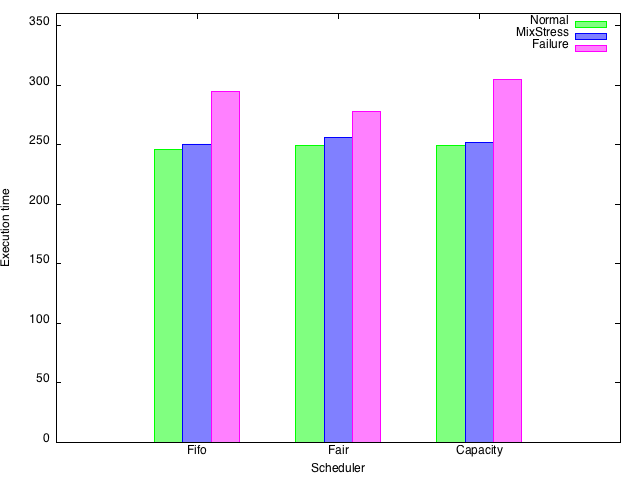
\includegraphics[width=1\linewidth]{failure_long.png}
  \caption{Execution time}
  \label{fig:failure}
\end{subfigure}%
\begin{subfigure}{.5\textwidth}
  \centering
  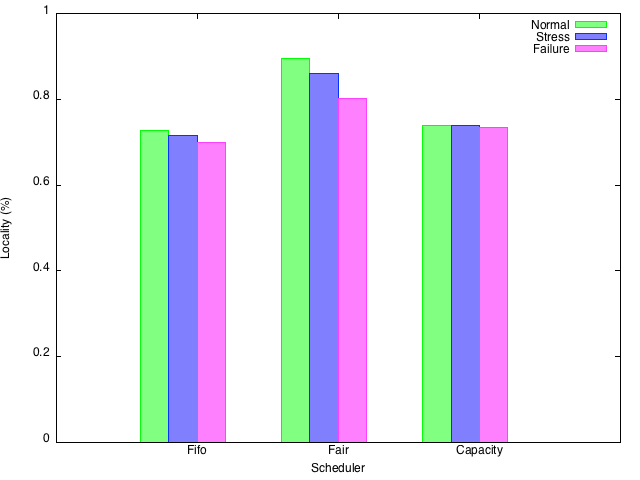
\includegraphics[width=1\linewidth]{localWFailure_long.png}
  \caption{Locality}
  \label{fig:localWFailure}
\end{subfigure}
\caption{Performance of Hadoop in 3 scenarios: Normal, Mix Stress and Failure}
\label{fig:test}
\end{figure}

Figure \ref{fig:failure} presents the total execution time in 3 different scenarios: Normal, Mix Stress and Failure in a cluster of 21 nodes with 6 Hadoop jobs of different sizes. In Normal scenario, we allow Hadoop run on dedicated nodes without introducing any stress or failure. The Mix Stress scenario has some CPU-intensive and IO-intensive processes launched on one node to simulate sporadic overloading situations. Failure scenario has 1 node fail after abitrarily 80 seconds (by simply killing the Task Tracker process running on that node). As we can see from Figure \ref{fig:failure}, stress slightly degrades Hadoop's performance a little, while failures prolong the execution of Hadoop jobs by a significant amount of time as much as 56 seconds (roughly 22.5\%) in case of Capacity scheduler.  Fair scheduler appears to suffer the least: its execution time is prolonged for only 29 seconds (10.4\%), and it also finishes the fastest among the three schedulers under failure (278 seconds compared to 294 seconds for FIFO, and 305 seconds for Capacity scheduler).


Figure \ref{fig:localWFailure} shows the percentage of locally executed tasks over the total number of tasks in the same scenarios. Fair scheduler still enjoys the highest number of locality, even though this number is decreasing. FIFO and Capacity scheduler shows some degradation, though this degradation is rather small compared to Fair scheduler (3\% and 1\% compared to 9\%). To explain this phenomenon, remember that Fair scheduler was designed based on the assumption that most tasks are short and therefore, nodes will release slot quickly enough for other tasks get locally executed. However, in case of failure, the long failure detection time (expiry time) creates the illusion of long-lasting tasks on failed node. These "fake" long tasks break the assumption of Fair scheduler, leading to high degradation.

\section{Related works}
There exists a problem regarding the failure handling mechanism of Hadoop that often gets overseen. When a task is declared failed, it gets "special treatment" in the manner that, failed tasks will be launched as soon as any slot becomes available, regardless of data locality. In a cluster where Data Node and Task Tracker processes co-reside, a machines failure will reduce the replication factor for those data splits originally on that node. Providing that Hadoop tries its best to provide locality for tasks in normal situation, it is likely that the failed tasks will have one less machine to run locally, which in turn leads to lower locality in general.

Providing locality for tasks is crucial for performance of Hadoop in large clusters because network bisection bandwidth becomes a bottleneck \cite{dean2008mapreduce}. Besides, since most of the Hadoop usage is for small jobs (jobs with small number of map tasks), it is difficult for a small job to obtain slots on nodes with local data. Data then has to be transferred through the network, which might significantly increase the execution time if network bandwidth is scarce. Providing locality for these jobs will greatly increase the performance of Hadoop in term of time and resource preserving.

Unfortunately, achieving high locality is not easy. Zaharia et al \cite{zaharia2010delay} introduces the Delay technique inside the Fair scheduler to improve locality of tasks. Instead of strictly following the order of jobs, Fair scheduler allows behind jobs launch their tasks first if the head-of-line job fails to launch a local task. However, Fair scheduler relies on the assumption that tasks are mostly short and slots are freed up quickly. In case of long tasks that occupy the slots, a node may not free up quickly enough for other jobs to achieve locality.

In the effort to overcome the above-mentioned problems, we propose preemption. Preemption allows a task to quickly release the slot for more urgent task. Locality can be assured with the employment of preemption. Also preemption allows the scheduler to have better control on the resources (i.e. the task slots) so that optimal efficiency can be obtained. Shorter tasks can preempt a longer one to achieve fast response time.

\subsection*{Preemption in Hadoop}
To our knowledge, there has been not much work aiming at providing the preemption feature for Hadoop:

Li Liu \cite{liu2012preemptive} introduces a Preemptive Deadline Constraint Scheduler (PDCS), which aims at minimizing the total completion time of jobs under deadlines. Traditional non-preemptive schedulers have to wait for previously assigned jobs’ completion or halt. This delays the execution of production jobs, sometimes renders them violating their deadlines. To avoid this, PDCS employs the Hadoop built-in preemption mechanism (kill) to provide slots for near deadline jobs. Upon submission, jobs are checked whether they can finish under its deadline or not using estimation. Jobs then are scheduled if the number of available slots meets the requirement. Otherwise, the scheduler would determine whether these jobs are legal to preempt the slots that have been already allocated.

Yandong Wang \cite{wang2013preemptive} introduces the Fair Completion Scheduler (FCS) that supports Reduce Task pre-emption. A long Reduce task would occupy the reduce slot, and significantly increase the completion time of shorter jobs. By check pointing the Reduce task, the reduce slot can be passed on to a different shorter job. After the short job finishes, the long Reduce task picks up the work from where it was left off, and continue until the end.

Pastorelli \cite{pastorelli2014assisted} proposes to leverage the already available POSIX signals such as \texttt{SIGTSTP} and \texttt{SIGCONT} to suspend running tasks. In Hadoop, Map and Reduce tasks are regular Unix processes running in child JVMs spawned by the TaskTracker. This means that they can safely be handled with the POSIX signaling infrastructure. The state of tasks is implicitly saved by the operating system, and kept in memory. If not enough physical memory is available for running tasks at any moment, the OS paging mechanisms saves the memory allocated to the suspended tasks in the swap area.

Pastorelli's approach save the state of the JVM and can be applied seamlessly to abitrary tasks regardless of types. However a suspended process can only be resumed on the same machine it was suspended on. If the same task gets scheduled on a different machine, it has to be restarted from scratch, losing work done so far: in that case, the \texttt{suspend} is effectively analogous to a delayed \texttt{kill}.

Although very interesting, the above mentioned efforts all suffer from some drawbacks. The Preemptive Deadline Constraint Scheduler approach employs the naive Kill primitive from Hadoop, which incurs a large amount of waste work. The Fair Completion Scheduler only concerns about preempting Reduce tasks but ignores the case of Map tasks. Pastorelli's OS-assisted preemptive primitives allow a seamless preemption mechanism for all types of tasks, but do not support migration, i.e. restarting the preempted tasks on a different node. These drawbacks limit the usage of these approaches. In the next chapter, we will discuss more about the choices between preemption styles, and our approach to overcome these drawbacks.



\section{Pause and Resume mechanism}
Preemption is a highly desirable feature in many cases. It allows schedulers to quickly reallocate resources between jobs for fair sharing. In other cases, preemption can reclaim resources from long running tasks and give them to shorter one. Providing local execution to short tasks helps reducing response time as well as lowering the network traffic between nodes in the same cluster. In this study, we introduce our preemption mechanism that is both fast and light-weight.

\subsection{Map task preemption}
Each Map task belonging to a Hadoop job is assigned a split of the data to process. Once all the input $<key,value>$ pairs have been processed, the Map task reports back to the Job Tracker, and the map output is entrusted to the local Task Tracker to serve to Reduce tasks.

Although the name is “pause and resume”, our Map preemption mechanism is inplemented in a structually different manner. There is no “pause” in Map task preemption, but we actually split the map tasks into 2 sub-tasks at the boundery between input $<key, value>$ pairs. The first sub-task covers all the map input $<key, value>$ pair that the task has processed so far. This sub-task is considered Completed and will report back to the Job Tracker as a normally completed task. The second sub-task includes all the map input $<key, value>$ pair that has not yet been processed. This sub-task will be treated as a new independent task with almost no difference compared to any other non-running tasks. The independence between $<key, value>$ pairs of the Map Reduce programming paradigm gurantees that our mechanism works correctly and does not produce any extra (or lose any) $<key, value>$ pair, thus ensuring correctness.

A Map task now does not simply loop through every single $<key, value>$ pair like in the original source code. At every $<key, value>$ pair, it needs to make sure the pair falls inside the task’s covering range. A simple comparison between starting key, ending key and the current key at each round serves the purpose. Besides, Map task now needs to actively listen to the signal from the Task Tracker in order to stop at any time. Finally, before committing the map output, Map task needs to mark the last processing input $ <key, value> $ pair, so the Job Tracker can know whether this task has completely finished or needs to be split into sub-tasks. Algorithm \ref{algo:mapTask} illustrates the new Map task’s workflow.

The creation of sub-tasks does not modify the underlying data split’s structure. Sub-tasks still require the same data split to process compared to its parental original task. This poses a drawback in our mechanism regarding the efficiency of data usage: the range of a sub-task might only cover, for example, 10\% of the data, but the same amount of data (1 chunk = 64 MB by default) will be required to transfer. It is then advisable not to split the task into too many small sub-tasks, as the network and computational waste would be high.

\subsection{Reduce task preemption}

A Reduce task is divided into 3 different phases. The Shuffle phase fetches all the segments that belong to it from intermediate Map Output data. The Sort phase performs a sort operation on all the fetches data, which was kept in $<key, value>$ pair format. Finally, the Reduce phase applies the user-defined reduce function on each of the Reduce-input $<key, value>$ pairs. Since the 3 phases are heavily dependent on each other, a similar “splitting” approach like in Map task preemption is unviable. We instead choose the traditional “pause and resume” approach where, at the moment of pausing, all the data of the Reduce task is stored in the local storage of the Task Tracker and, at the moment of resuming, data is loaded back to the memory.

Our mechanism allows a Reduce task to preempt itself at any time during the course of the Shuffle phase, and at the boundery of other phases. The Sort phase is usually very short due to the fact that Hadoop launches a separate thread to merge the data as soon as they become available. Preempting Reduce task during Reduce phase is also feasible, however we will consider this in future work.

\subsubsection{Pause}
During the Shuffle phase, a Reduce task fetches all the segments that belong to it from all intermediate map outputs. According to the sizes of the segments, Reduce Task stores them either to local disks or in memory. Meanwhile, multiple merging threads merge fetched data into larger segments and store them in an ordered structure that later can be popped out to feed to Reduce function. Preserving the state of Shuffle phase means to keep track of the shuffling status of all segments. Upon receiving preemption request, Reduce task stops all the fetching and merging thread gracefully: it allows the threads to finish the last unit of work they are currently on. Fetching threads can finish fetching the last segment of Map output, while Merging threads can finish merging the current segment.

After stopping all communication and sorting threads, the Reduce task flushes all the in-memory data to the disks while leave all the on-disk segments untouched. In-memory data includes in-memory segments and other data to keep track of the progress (number of copied segments, number of sorted segments...). These data is kept in files stored in each task attempt’s specific folder so that later re-launched attempt can access to these files and resume operation.

Preemption at the phases’ boundery follows exactly the same procedure. Data is flushed to disks, and all the information needed to re-create the running task is also stored in files. After that, the Reduce task preempts itself and releases the slot. The task reports back to the Job Tracker with a new status of “SUSPENDED”. Suspended task will go through almost the same procedure as Failed task, except increasing the count for failed tasks. It is also added back to the pool for later resume.

\subsubsection{Resume}

The information about the previously launched Task Tracker is stored inside the task. Upon re-launch, the Reduce task checks to see if it has been launched somewhere before. The location can be either local (task is re-launched on the same Task Tracker) or remote (task is re-launched on a different Task Tracker). The task then tries to fetch the already processed data from the previously launched Task Tracker before resuming to the point where it left off.

Our mechanism is incremental in the sense that it allows the task to be preempted multiple times. However, we do not allow the re-launched task to be preempted during the period when it fetches data from previously launched Task Tracker. Task needs to finish resuming to the previous state before being able to be preempted again. This is to prevent having flushed data on too many Task Trackers, which will make the resuming process complex and inefficient.

\section {Preemptive locality-driven scheduler}
In order to demonstrate the effectiveness of out new mechanism, we design a new scheduler, namely the Preemptive Locality-driven scheduler (PLS), that employs this new option to provide better locality for Map Reduce jobs. In normal situations without any failure, PLS behaves similarly to the default FIFO scheduler of Hadoop. However, when failures occur, PLS actively leverages the preemption mechanism to provide local execution for failed tasks.

Upon a task’s failure, PLS assembles a list of Task Trackers that has local data to the failed task (if it was of Map type), or simply list of all running Task Trackers (if it was of Reduce type).  If any of these task trackers has a free slot of the right task type, PLS simply allows the task to be launched from that task tracker at the next heartbeat. If no free slot is found, PLS tries to find appropriate task from all the currently running tasks on those task trackers to preempt. Figure \ref{algo:preemptiveFifo} illustrates the logic of finding a task to preempt:
\begin{algorithm}[!h]
\caption{Finding a task to preempt}
\label{algo:preemptiveFifo}
\begin{algorithmic}
\STATE {/*get the list of all suitable Task Trackers*/}
\STATE List taskTrackers = getListOfTaskTracker();
\STATE {/*get the list of all tasks running on those task trackers*/}
\STATE List tasks = getListStatusesOfTasks(taskTrackers);
\STATE {/*sort the tasks in the reverse job order*/}
\STATE tasks.sort();
\FOR {\{Task {\bf t} : tasks\} }
\IF{( {\bf t} belongs to jobs of lesser priority
\\ \indent {\bf AND} {\bf t}.progressScore $<$ {\bf THRESHOLD}
\\ \indent {\bf AND} !t.isCleanUp() {\bf AND} !t.isSetUp()
\\ \indent {\bf AND} !preemptList.contains(t)}
\STATE preempt\_task(t);
\STATE preemptList.add(t);
\STATE {\bf return};
\ENDIF
\ENDFOR
\end{algorithmic}
\end{algorithm}

PLS only allows failed tasks to preempt tasks from later submitted jobs. To respect the FIFO order, PLS prioritizes preempting tasks that belong to the latest submitted jobs. However, not all tasks would be considered for preemption. Preempting a task at, for example, 0.99 progress score would not be advisable, as it only introduces unnecessary waste which is more costly than waiting for that task to end (and perhaps the task will be already completed by the time of the next heartbeat). We impose a THRESHOLD of progress score so that almost complete tasks will not be considered for preemption. This THRESHOLD value is configurable via mapred-site.xml file, and the default value is set to 0.8.

In case PLS cannot find any task to preempt (for example, tasks all belong to the same or higher priority jobs, or all tasks are close to completion), PLS let the task to be launched at any arbitrary Task Tracker that has free slot the earliest. This is similar to the original FIFO scheduler’s procedure. This is to avoid having to wait for too long for a local slot.

\section{Evaluation}
In order to prove the efficiency of Pause and Resume preemption mechanism, we present the result from selected experiments. The goal is to demonstrate how the Preemptive Locality-driven scheduler manages to help jobs under failures. For this purpose, we concern about the execution time of jobs that suffer the failure, as well as their localities.

We performed our experiment on Grid5000 testbed, with a cluster of 21 nodes (1Master and 20 Slave nodes). Each node has 2 Map and 2 Reduce slots. Replication factor is set to 2. For timely reason, expiry time is set at 30 seconds. Speculation is turned off for correct evaluation of Pause and Resume mechanism's effeciency.

\subsubsection*{Jobs}
For simplicity, we only run 2 jobs of WordCount application with the same input size of 30GB. Failure is injected at 150 seconds to maximize the number of failed tasks from job 1.

\subsection*{Execution time}
\begin{figure}[ht]
    \centering
    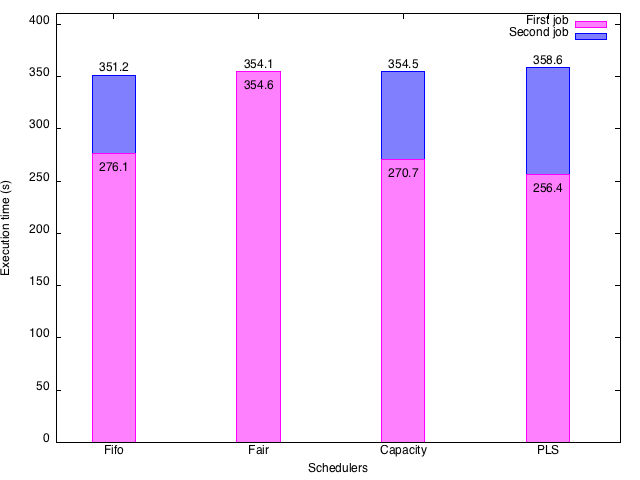
\includegraphics[width=1\linewidth]{time.png}
    \caption{Finish time of jobs with different schedulers}
    \label{fig:finalTime}
\end{figure}

Figure \ref{fig:finalTime} shows the finishing time of each job in the 4 different schedulers: the three readily available schedulers of Hadoop (FIFO, Fair and Capacity scheduler) and Preemptive Locality-driven scheduler (PLS). There is little difference in the total execution time of the two jobs (represented by the finishing time of the seconds job), but the trend is that PLS has to pay the most time to finish the set of jobs. However, PLS shows good improvement in the finishing time of job 1 - the job that suffers from the failure. PLS only requires 256.4 seconds to finish job 1, roughly 14 seconds (5.2\%) faster than in Capacity and about 20 seconds (7.2\%) when compare to FIFO scheduler. Fair scheduler performs poorly on this metrics, as jobs share the resources of the cluster. In fact, job 1 takes more time to finish than job 2 does in Fair scheduling. This can be explained by the fact that job 1 starts first and has more failed tasks than job 2.

To further understand about the efficiency of PLS, as well as the actual behavior of Pause and Resume preemption feature, we perform the same experiment with 3 different flavors of PLS. We omit completely the preemption function of PLS and mimic the FIFO scheduler in a flavor called FIFO*. FIFO* still has to pay the overhead of allowing Pause and Resume at any time (this overhead will be discussed later). The Kill-PLS uses the Kill primitive provided by Hadoop instead of Pause and Resume. Finally, the PLS that leverages the Pause and Resume function is also included.

\begin{figure}[ht]
    \centering
    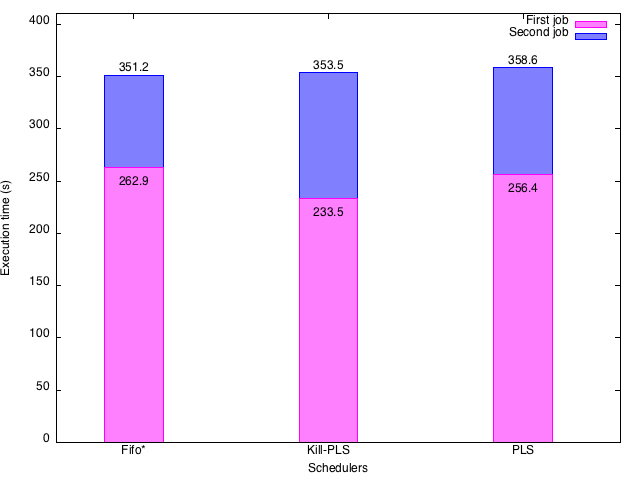
\includegraphics[width=1\linewidth]{mod.png}
    \caption{Execution with different flavors of PLS}
    \label{fig:flavors}
\end{figure}

Figure \ref{fig:flavors} compares the execution of Hadoop with different flavors of PLS. The FIFO* enjoys the best performance due to the fact that there is no killing or preemption overhead. Tasks are launched and finish naturally without any waste work (from killing) or delay (from splitting and re-launching a task).

Though witnessing some degradation in the total performance, Kill-PLS and PLS gain some improvement in term of Job 1's execution time. Both of Kill and Preemption finish the first job faster than that of FIFO*, in the order of roughly 19 (11.2\%) and 7 (2.5\%) seconds, respectively. Kill-PLS outperforms the other 2 competitors thanks to the fact that kill command can instantly rescue the slots from currently running tasks, while preemption command needs to pay some delay so that running tasks can save the states and release the slots. However, PLS manages to save some work from preempted tasks. PLS only requires an extra 102 seconds to finish the second job, compared to 120 seconds in Kill-PLS (an improvement of 15\%).

\subsection*{Data locality of the first job}
\begin{figure}[ht]
    \centering
    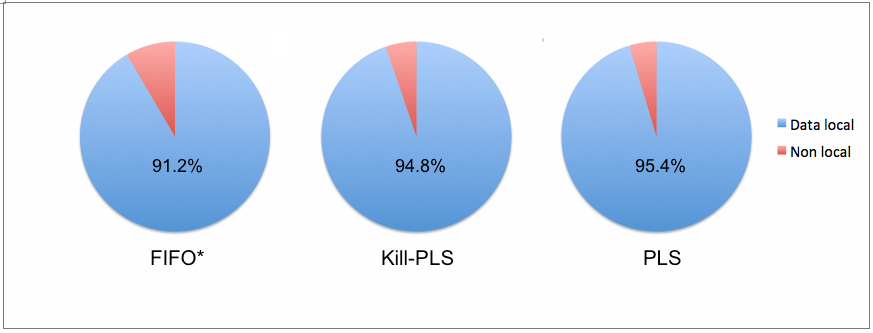
\includegraphics[width=1\linewidth]{flavorLocality.png}
    \caption{Locality of the first job}
    \label{fig:finalLocality}
\end{figure}

Figure \ref{fig:finalLocality} shows the locality of the first jobs in the three different flavors. FIFO* has the lowest value of data locality (90.4\%) due to the fact that failed tasks are assigned regardless of locality. Kill-PLS and PLS observe higher locality in Map tasks and equal each other with the values of 94.8\% and 95.4\%, respectively. This means PLS manages to improve the locality of Map tasks by almost 5\%. Out of 12 failed tasks (tasks that were initially launched on the failed node), FIFO* assigns all 12 tasks remotely (rack-locally), while Kill-PLS and PLS assigns only 3 remotely (as in table \ref{table:failedlocality}).
\begin{center}
\begin{table}[h]
\centering
    \begin{tabular}{ | >{\centering}p{4cm} | >{\centering}p{4cm} | >{\centering\arraybackslash}p{4cm} |}
    \hline
	FIFO* & Kill-PLS & PLS \\ \hline
    0/12 (0\%)& 9/12 (75\%) & 9/12 (75\%)   \\ \hline
    \end{tabular}
    \caption{Number of local re-executed tasks}
    \label{table:failedlocality}
\end{table}
\end{center}

\section{Conclusion}
This thesis addresses the problem by investigating the fault-tolerance mechanism of Hadoop, a popular implementation of MapReduce. It presents some results to illustrate Hadoop's behaviors under different situations. The intent was to confirm the mechanism and analyze the drawbacks of how Hadoop handles failures.

We proposed the designed of a new feature for Hadoop: the waste-free preemption function. By allowing a task to preserve its state and release the slot in a timely manner, Hadoop can have more control over resources. This in turn will help increase the performance of Hadoop under the occurrence of failure. The preemption feature was implemented not only with the intention of improving performance under failure, but also to open new possibilities for further improvement under other circumstances.

Finally, we evaluated the effectiveness of the new feature considering some basics metrics such as execution time and data locality. In this work, we compare the original Fifo scheduler with a preemptive version. Experiments show that our new feature improves the execution time of Hadoop job when failure occurs. Although the preemption mechanism imposes some overhead, if wisely used, it can greatly improve Hadoop's performance.

\subsection*{Future work}
Our work suffers from some concerns regarding the usability, as well as efficiency. Firstly, the Reduce Pause and Resume mechanism should be further extended to allow preemption during Reduce phase. This allows a more fine-grain control over Reduce tasks. Secondly, it would be interesting to evaluate the cost of preempting a Reduce task, in comparison with Killing. Killing instantly releases the slot, but wastes the effort, while Preemption may take sometime before the slot is released. Also, upon resuming, Reduce tasks also require some extra time to load up the data from the local storage. These two delays add up and in some cases, it is more beneficial to decide to Kill rather than Preempt a Reduce task.

\bibliography{reference}

\begin{thebibliography}{4}

\bibitem{borthakur2008hdfs} Borthakur, Dhruba. "HDFS architecture guide." HADOOP APACHE PROJECT http://hadoop. apache. org/common/docs/current/hdfs design. pdf (2008).

\bibitem{ghemawat2003google} Ghemawat, Sanjay, Howard Gobioff, and Shun-Tak Leung. "The Google file system." ACM SIGOPS Operating Systems Review 37, no. 5 (2003): 29-43.

\bibitem{shvachko2010hdfs} Shvachko, Konstantin V. "HDFS Scalability: The limits to growth." login 35, no. 2 (2010): 6-16.

\bibitem{shvachko2010hadoop} Shvachko, Konstantin, Hairong Kuang, Sanjay Radia, and Robert Chansler. "The hadoop distributed file system." In Mass Storage Systems and Technologies (MSST), 2010 IEEE 26th Symposium on, pp. 1-10. IEEE, 2010.

\bibitem{white2012hadoop} White, Tom. "Hadoop: The definitive guide." (2012).

\bibitem{welcomepage}Apache Hadoop Welcome page, \url{http://http://hadoop.apache.org}

\end{thebibliography}

\end{document}
